\documentclass[ngerman]{beamer}


\usepackage[utf8]{inputenc}
\usepackage[T1]{fontenc}
\usepackage{booktabs}
\usepackage{babel}
\usepackage{graphicx}
\usepackage{csquotes}
\usepackage{xcolor}

\author{Dr. Uwe Ziegenhagen}
\title{Grundlagen der Einkommenssteuer in Deutschland}

\begin{document}

\begin{frame}

\maketitle

\end{frame}

\begin{frame}
\frametitle{Disclaimer}

\begin{itemize}
\item Ich bin kein Steuerfachmann
\item Alle Angaben auf Basis besten Wissens und Gewissens
\item Sämtliche Angaben in dieser Präsentation ohne Gewähr, kein Anspruch auf Vollständigkeit
\item Für rechtssichere Auskünfte geht zum Steuerberater oder Finanzamt
\item Thema ist komplex $\Rightarrow$ 10--15\% der Weltsteuerliteratur kommt aus Deutschland
\end{itemize}
\end{frame}


\begin{frame}
\frametitle{Inhalt}

\tableofcontents

\end{frame}

\section{Grundlagen}

\begin{frame}
\frametitle{Rechtsgrundlagen}
\framesubtitle{~}

\begin{itemize}
\item Basis für die Erhebung der Einkommenssteuer: EStG (\url{https://www.gesetze-im-internet.de/estg/inhalts_bersicht.html})
\item §1 EStG: \enquote{Natürliche Personen, die im Inland einen Wohnsitz oder ihren gewöhnlichen Aufenthalt haben, sind unbeschränkt einkommensteuerpflichtig.}

\begin{itemize}
	\item Natürliche Personen: Menschen, keine juristischen Personen
	\item Unbeschränkte Steuerpflicht beginnt mit der Geburt bzw. dem Zuzug, endet mit dem Tod bzw. dem Wegzug!
	\item Beschränkt: für Leute, die keinen Wohnsitz haben und sich <183 Tage in Deutschland aufhalten
\end{itemize}
\end{itemize}
\end{frame}

\begin{frame}
\frametitle{Wer muss eine Steuererklärung abgeben?}
\framesubtitle{~}

\begin{description}
\item[Pflichtveranlagung] Man muss eine Steuererklärung abgeben.
\item[Antragsveranlagung] Man gibt freiwillig eine Steuererklärung ab\footnote{spätestens 4 Jahre nach Ende des Steuerjahres}
\end{description}

\textbf{Abgabepflicht}

\begin{itemize}
	\item Wer verpflichtet ist, muss Erklärung bis 31. Mai des Folgejahres abgeben
	\item ab 2019: zum 31. Juli
	\item Sonst böser Brief mit Hinweis auf §~328 AO (Zwangsgelder), §~162 AO (Schätzung) oder \enquote{weitere Maßnahmen}, z.B. §~152 AO (Verspätungszuschlag)
	\item Abgabepflicht für Arbeitnehmer in §~46 EStG (\url{http://www.gesetze-im-internet.de/estg/__46.html})
\end{itemize}

\end{frame}



\begin{frame}
\frametitle{Progression}
\framesubtitle{~}

\begin{itemize}
\item Steuerprogression: Ansteigen des Steuersatzes in Abhängigkeit vom zu versteuernden Einkommen oder Vermögen. 
\item $\Rightarrow$ Wer mehr verdient, zahlt proportional mehr Einkommenssteuer!
\item fünf Zonen (Zahlen für 2017) mit jeweils anderen Parametern für die Steuerberechnung
\end{itemize}


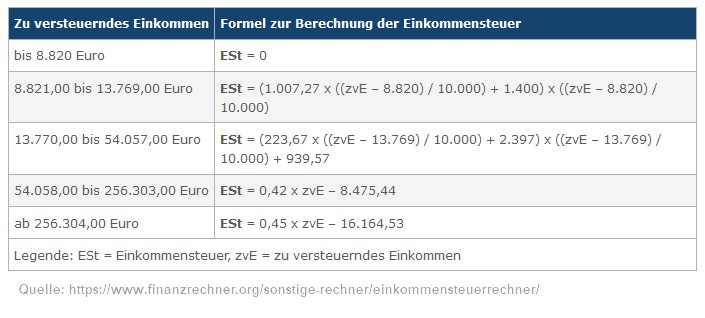
\includegraphics[width=\textwidth]{Bilder/Formeln}

\end{frame}

\begin{frame}
\frametitle{Progression}
\framesubtitle{~}

\textbf{Begriffe}

\begin{description}
\item[Grenzsteuersatz] Mit wieviel \% wird der nächste Euro Einkommen versteuert?
\item[Durchschnittssteuersatz] Wieviel \% des Einkommens gehen für die ESt drauf?
\item[Kalte Progression] Steuermehrbelastung wenn die Variablen eines progressiven Steuertarifes nicht an Inflation angepasst werden.
\end{description}

Beispiel: Jahreseinkommen von 8821 Euro: 8820 Euro sind steuerfrei, nur für den 8821en Euro fallen 0.14 Euro Steuern an.



\end{frame}

\begin{frame}
\frametitle{Einkommen}
\framesubtitle{~}

Sieben Einkommensarten:

\begin{enumerate}
\item Einkünfte aus nichtselbständiger Arbeit (§ 19 EStG)
\item Einkünfte aus Kapitalvermögen (§ 20 EStG)
\item Einkünfte aus Vermietung und Verpachtung (§ 21 EStG)
\item Sonstige Einkünfte (§ 22, § 23 EStG)
\item Einkünfte aus Land- und Forstwirtschaft (§ 13, § 13a, § 14, § 14a EStG)
\item Einkünfte aus Gewerbebetrieb (§ 15, § 16, § 17 EStG)
\item Einkünfte aus selbständiger Arbeit (§ 18 EStG)
\end{enumerate}

1--4 sind \enquote{Überschusseinkünfte}, 5--7 

\end{frame}

\begin{frame}
\frametitle{Überschusseinkünfte \& Gewinneinkünfte}
\framesubtitle{~}

\begin{description}
\item[Überschusseinkünfte] Überschusseinkünfte im deutschen Einkommensteuerrecht sind Einkünfte, die nach § 2 Abs. 2 Nr. 2 EStG als Überschuss der Einnahmen über die Werbungskosten berechnet werden
\item[Gewinneinkünfte] Gewinneinkünfte im deutschen Einkommensteuerrecht sind Einkünfte, bei denen nach § 2 Abs. 2 Nr. 1 EStG die Einkünfte dem Gewinn entsprechen. 
\end{description}

\end{frame}


% https://de.wikipedia.org/wiki/Gewinneink%C3%BCnfte


\end{document}